\documentclass{article}

\usepackage{graphicx}
\usepackage{tikz}
\usepackage{tikzsymbols}
\usetikzlibrary{calc,patterns,shapes.geometric}
\pagestyle{empty}
\usepackage[margin=0pt]{geometry}
\geometry{papersize={14in,12in}}

\def\centerarc[#1](#2)(#3:#4:#5){\draw[#1] ($(#2)+({#5*cos(#3)},{#5*sin(#3)})$) arc (#3:#4:#5);}

\begin{document}
	\begin{figure}
		\centering
		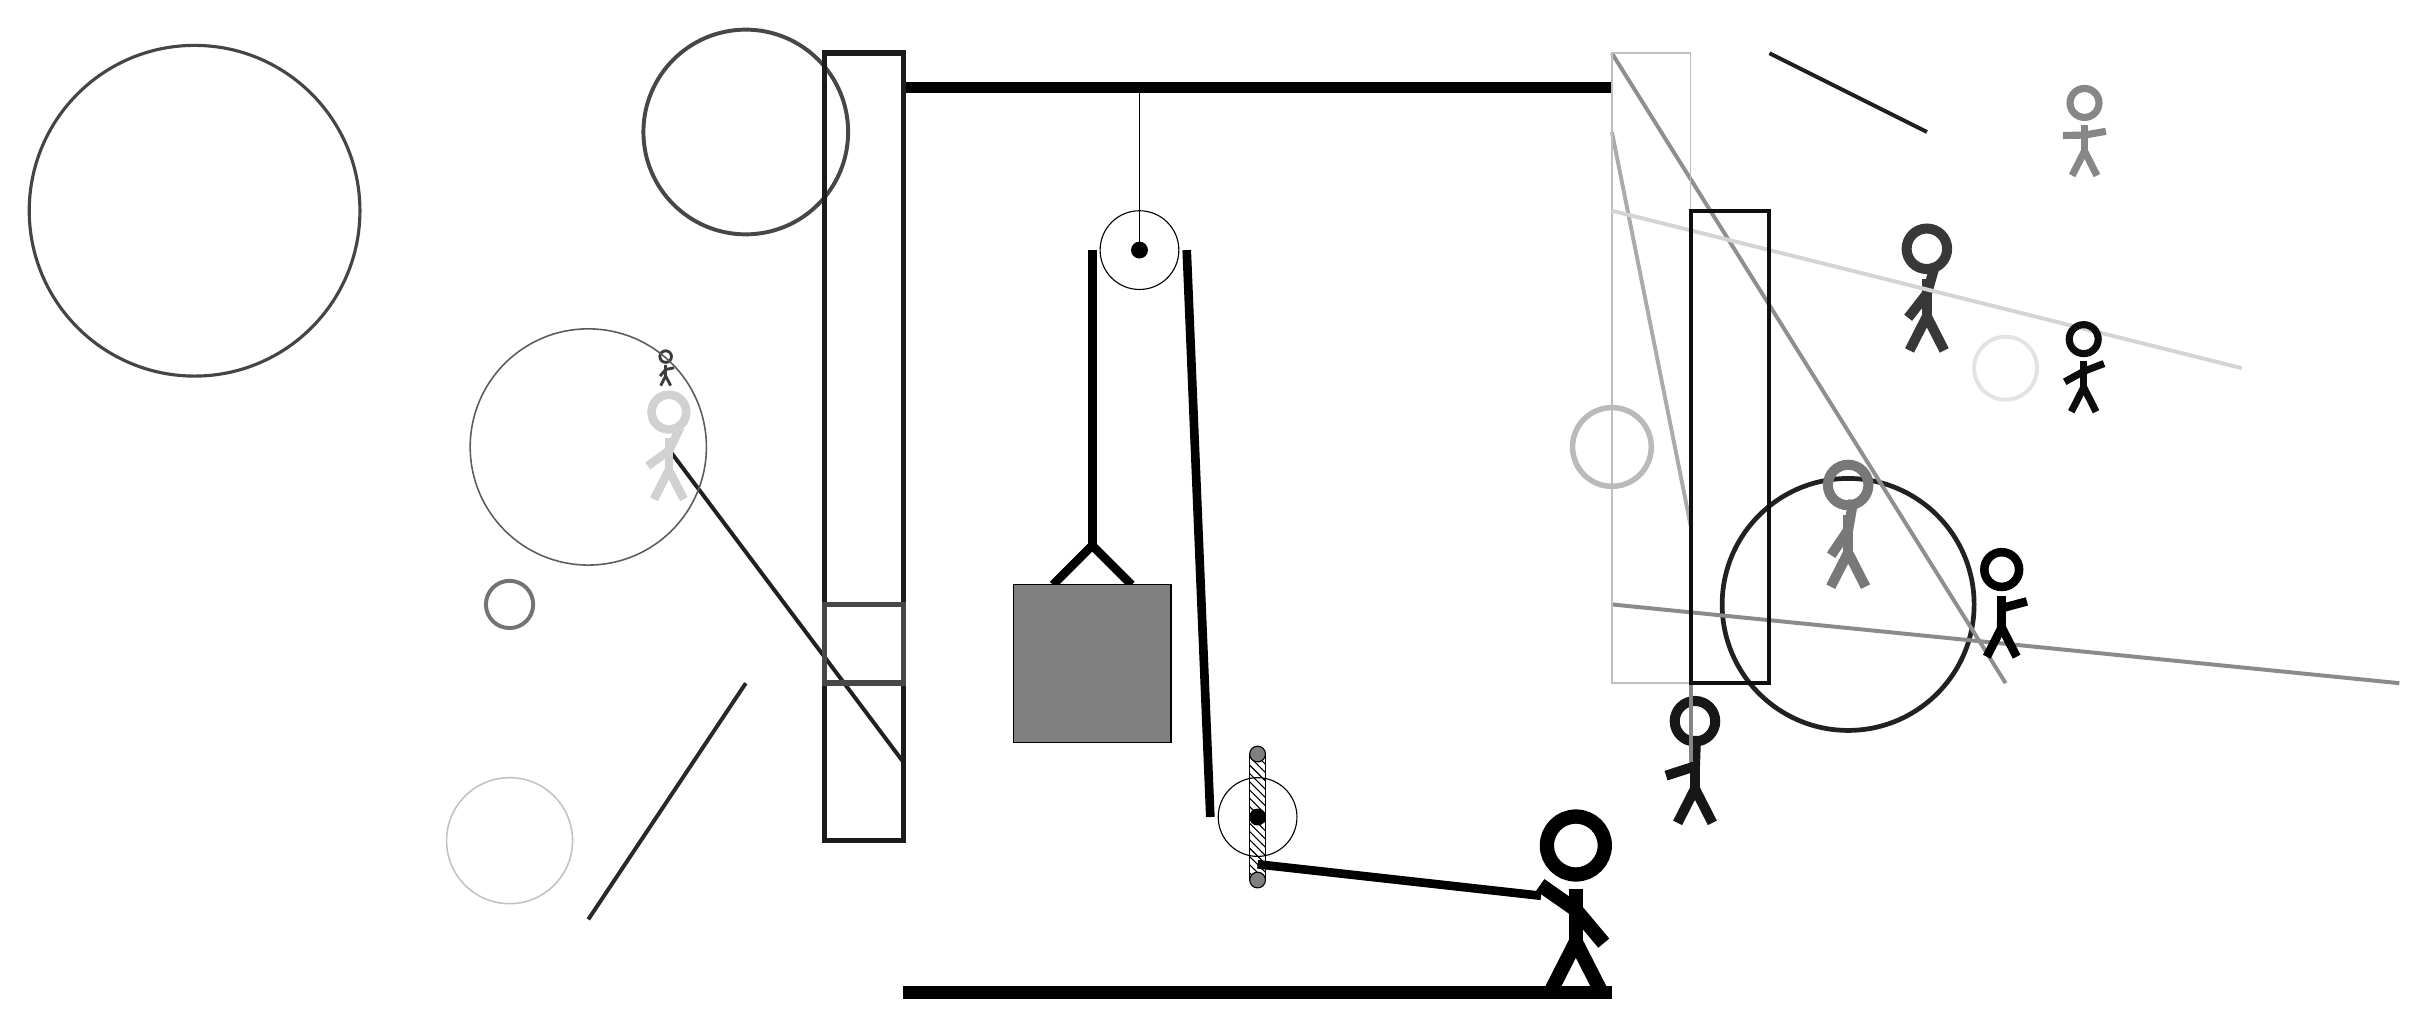
\begin{tikzpicture}
			%%%%% START %%%%%
			
			\draw[fill=black] (-2, 11.5) rectangle (7, 11.625);
			
			\draw (1, 9.5) circle (0.5);
			\draw[fill=black] (1, 9.5) circle (0.1);
			\draw (1, 11.5) -- (1, 9.5);
			
			\draw[fill=white](2.5, 2.3) circle (0.5);
			\draw[fill=black] (2.5, 2.3) circle (0.1);
			\draw[pattern=north west lines, pattern color=black] (2.4, 3.1) rectangle (2.6, 1.5);
			\draw[fill=black!50] (2.5, 3.1) circle (0.1);
			\draw[fill=black!50] (2.5, 1.5) circle (0.1);
			
			\draw [line width=0.5mm, color=black!11](12, 8) circle (0.4);
			
			\node[line width=0.7mm, color=black!47] at (13, 11) {\Strichmaxerl[5][1][10]};
			\node[line width=0.2mm, color=black!78] at (11, 9) {\Strichmaxerl[7][52][74]};
			\draw [line width=0.5mm, color=black!55](-7, 5) circle (0.3);
			\node[line width=0.4mm, color=black!77] at (-5, 8) {\Strichmaxerl[2][50][11]};
			\draw[line width=0.5mm, color=black!33](8, 6) -- (7, 11);
			\draw [line width=0.2mm, color=black!24](-7, 2) circle (0.8);
			\draw[line width=0.5mm, color=black!87](-5, 7) -- (-2, 3);
			\draw [line width=0.4mm, color=black!73](-11, 10) circle (2.1);
			
			\draw [line width=0.6mm, color=black!87](10, 5) circle (1.6);
			
			\node[line width=0.7mm, color=black!18] at (-5, 7) {\Strichmaxerl[6][36][64]};
			\draw[line width=0.5mm, color=black!46](7, 5) -- (17, 4);
			\draw[line width=0.5mm, color=black!44](7, 12) -- (12, 4);
			
			\draw[line width=0.2mm, color=black!25] (7, 12) rectangle (8, 4);
			\node[line width=0.4mm, color=black!100] at (12, 5) {\Strichmaxerl[6][88][15]};
			\draw[line width=0.5mm, color=black!17](7, 10) -- (15, 8);
			
			\node[line width=0.5mm, color=black!53] at (10, 6) {\Strichmaxerl[7][56][80]};
			
			\draw [line width=0.5mm, color=black!72](-4, 11) circle (1.3);
			\draw[line width=0.7mm, color=black!89] (-2, 12) rectangle (-3, 2);
			\draw[line width=0.5mm, color=black!88](9, 12) -- (11, 11);
			\draw[line width=0.5mm, color=black!84](-4, 4) -- (-6, 1);
			
			\node[line width=0.3mm, color=black!91] at (8, 3) {\Strichmaxerl[7][18][88]};
			
			\draw[line width=0.5mm, color=black!48](8, 5) -- (8, 3);
			\draw[line width=0.7mm, color=black!72] (-2, 5) rectangle (-3, 4);
			\draw [line width=0.7mm, color=black!27](7, 7) circle (0.5);
			
			\draw [line width=0.2mm, color=black!64](-6, 7) circle (1.5);
			\node[line width=0.5mm, color=black!95] at (13, 8) {\Strichmaxerl[5][29][21]};
			\draw [line width=0.3mm, color=black!67](-3, 5) circle (0.0);
			\draw[line width=0.5mm, color=black!94] (8, 4) rectangle (9, 10);
			
			
			\draw[line width=1.1mm] (-0.1, 5.25) -- (0.4, 5.75) -- (0.9, 5.25);
			\draw[fill=black!50] (-0.6, 5.25) rectangle (1.4, 3.25);
			
			\draw[line width=1.1mm] (0.4, 9.5) -- (0.4, 5.75);
			\centerarc[line width=1.1mm](1, 9.5)(0:180:0.6);
			\draw[line width=1.1mm](1.6, 9.5) -- (1.9, 2.3);
			\centerarc[line width=1.1mm](2.5, 2.3)(180:270:0.6);
			\draw[line width=1.1mm](2.5, 1.7) -- (6.1, 1.3);
			
			\node at (6.5, 1.2) {\Strichmaxerl[10][-35][-50]};
			
			\draw[fill=black] (-2, 0) rectangle (7, 0.15);
			
			%%%%% END %%%%%
		\end{tikzpicture}
	\end{figure}	
\end{document}